\documentclass[a4paper, UTF8]{ctexrep}
\usepackage{ctex}
\usepackage{amsmath}
\usepackage{multirow}
\usepackage{amssymb}
\usepackage{graphicx}
\usepackage{geometry}
\usepackage{bm}
\usepackage{subfigure}
\usepackage{float}

\renewcommand\thesection{\arabic{section}}

\begin{document}
	\begin{titlepage}
		\centering
		\vspace{6cm}
		\LARGE{图像处理中的数学方法第二次作业报告}\\
		\vspace{3cm}
		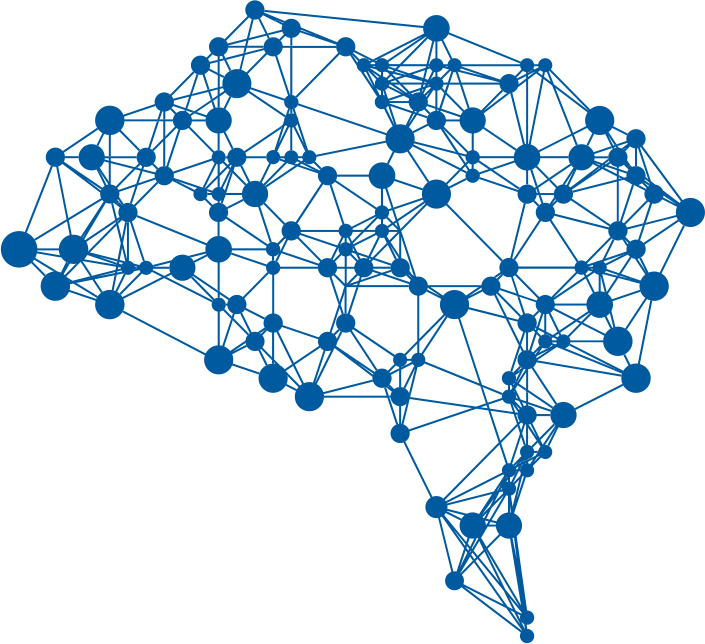
\includegraphics[width=0.8\textwidth]{deepLearning.png}\\
		\vspace{4cm}
		\normalsize{安捷 1601210097}\\
		\normalsize{\today}
	\end{titlepage}
	为了实现本次作业的需求,我基于MATLAB,实现了以下三种算法:
	\begin{enumerate}
		\item Heat Equation Denoising
		\item Perona Malik Denoising
		\item Shock Filter Deblur
	\end{enumerate}
	并且,分别针对前两种算法尝试了不同的演化时间(即离散情况下的迭代次数)下的算法效果;针对第三种算法尝试了不同的噪声水平、采用不同的L算法以及长时间演化下算法的效果。
		\section{参数设置}
			\subsection{heat\_equation\_denoise参数设置}
				\begin{table}[htbp!]
					\centering
					\begin{tabular}{cc}
						\hline
						参数名称 & 参数值 \\
						\hline
						MAX\_ITERATION & 100/200/300/500 \\
						NOISE\_SCALE & 100 \\
						DISCRETE\_TIME & 0.05 \\
						\hline
					\end{tabular}
					\caption{heat\_equation\_denoise参数表}
				\end{table}
				其中,噪声的添加方式与上一次作业相同,这里的NOISE\_SCALE参数即为上一次作业中噪声赋值的参数,DISCRETE\_TIME为每次演化时的时间长度。
			\subsection{perona\_malik\_denoise参数设置}
				\begin{table}[htbp!]
					\centering
					\begin{tabular}{cc}
						\hline
						参数名称 & 参数值 \\
						\hline
						MAX\_ITERATION & 100/200/300/500 \\
						NOISE\_SCALE & 100 \\
						DISCRETE\_TIME & 0.05 \\
						K & 0.05 \\
						\hline
					\end{tabular}
					\caption{perona\_malik\_denoise参数表}
				\end{table}
			\subsection{shock\_filter\_deblur参数设置}
				\begin{table}[htbp!]
					\centering
					\begin{tabular}{cc}
						\hline
						参数名称 & 参数值 \\
						\hline
						MAX\_ITERATION & 200/500 \\
						NOISE\_SCALE & 100/200/100000 \\
						DISCRETE\_TIME & 0.01 \\
						SIGMA & 2 \\
						\hline
					\end{tabular}
					\caption{shock\_filter\_deblur参数表}
				\end{table}
				其中,SIGMA为Gauss平滑算子的标准差。
			\section{数值实验结果}
				我按照上述参数表中的设定分别进行了若干组数值实验,现将熟知实验的结果展示如下:
				\begin{figure}[htbp!]
					\centering
					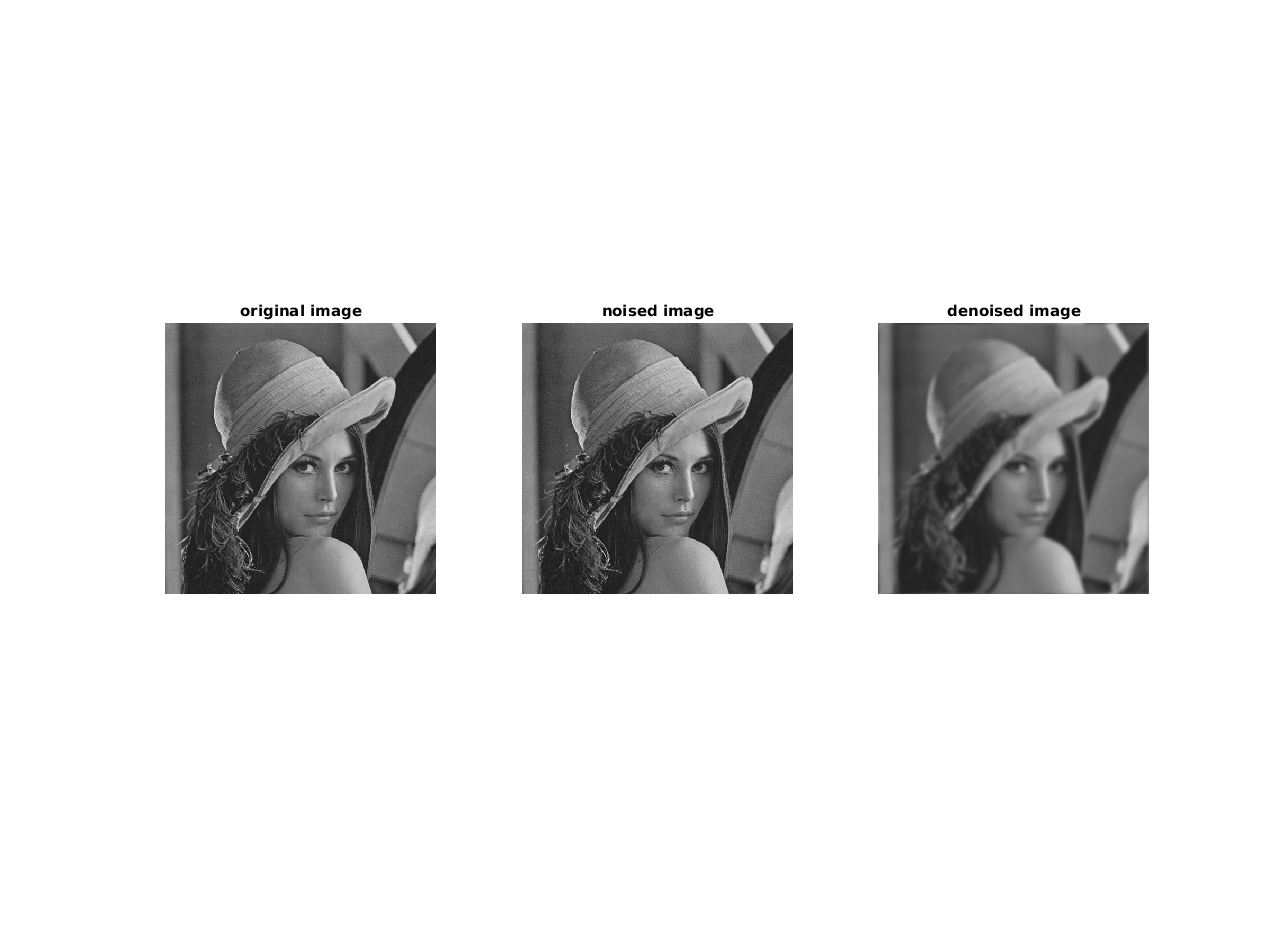
\includegraphics[width=0.8\textwidth]{hw2_fig1.png}
					\caption{heat\_equation\_denoise数值实验结果}
					\label{}
				\end{figure}
				\begin{figure}[htbp!]
					\centering
					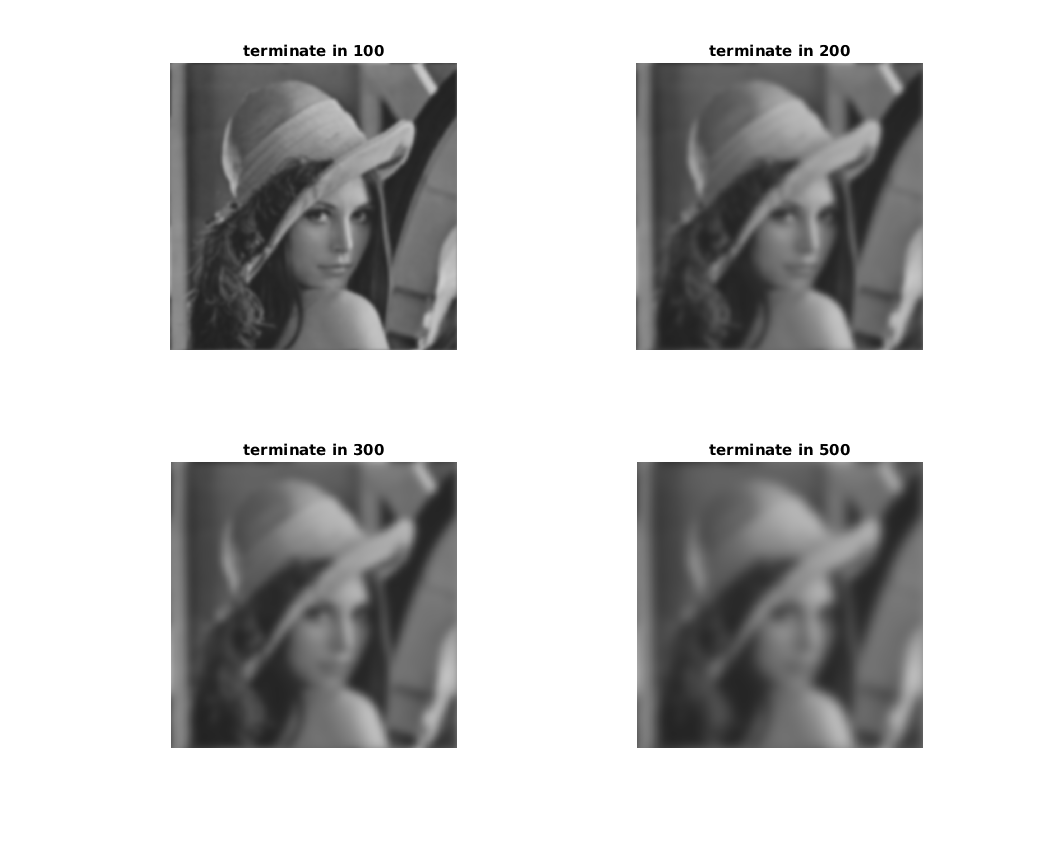
\includegraphics[width=0.8\textwidth]{hw2_fig2.png}
					\caption{heat\_equation\_denoise数值实验结果}
					\label{}
				\end{figure}
				\begin{figure}[htbp!]
					\centering
					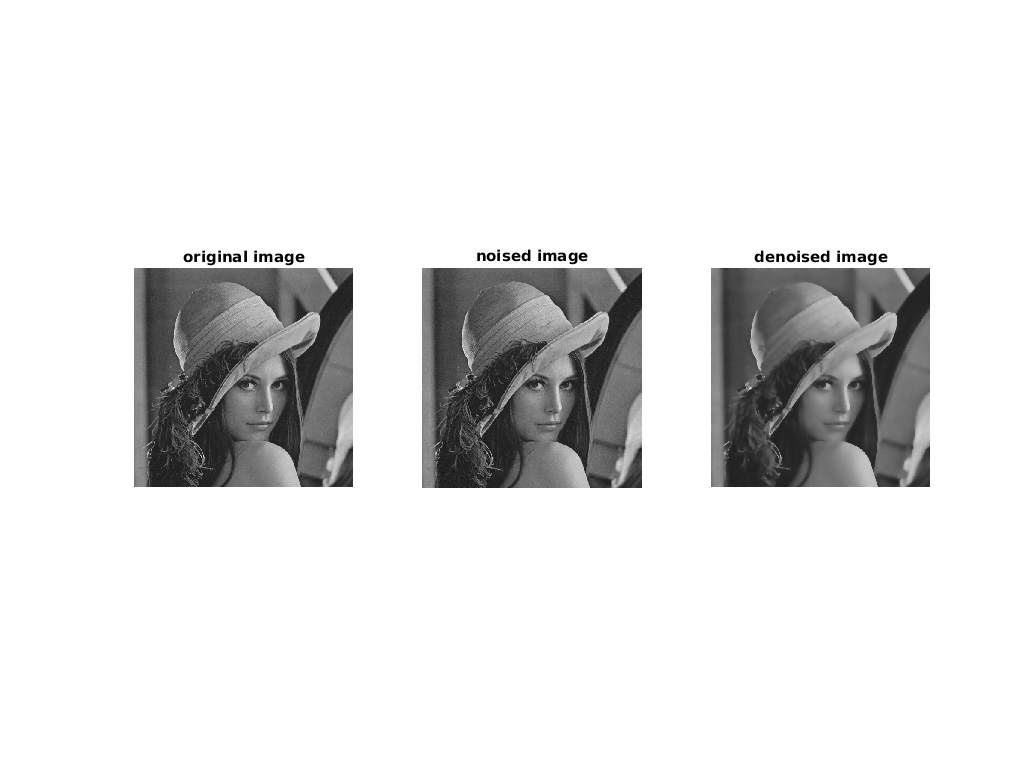
\includegraphics[width=0.8\textwidth]{hw2_fig3.png}
					\caption{perona\_malik\_denoise数值实验结果}
					\label{}
				\end{figure}
				\begin{figure}[htbp!]
					\centering
					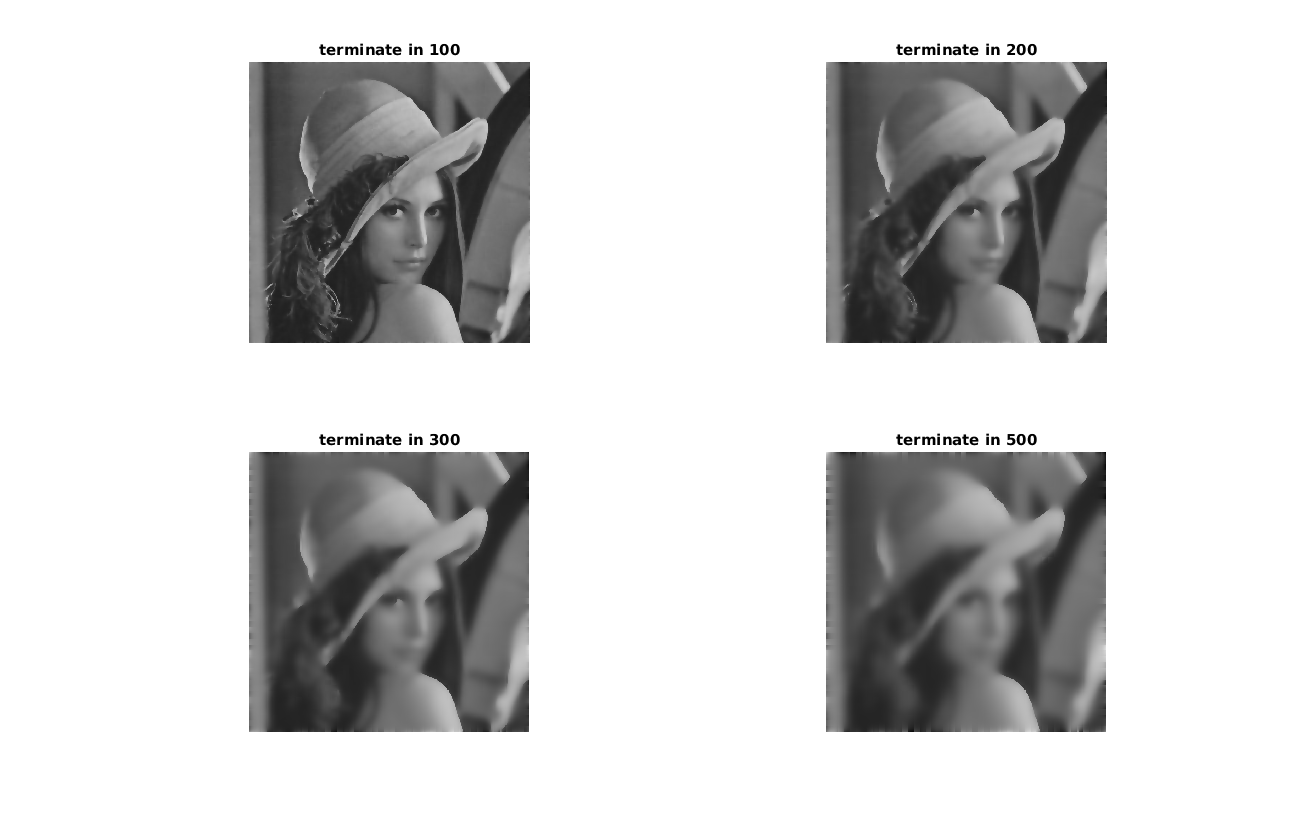
\includegraphics[width=0.8\textwidth]{hw2_fig4.png}
					\caption{perona\_malik\_denoise数值实验结果}
					\label{}
				\end{figure}
				\begin{figure}[htbp!]
					\centering
					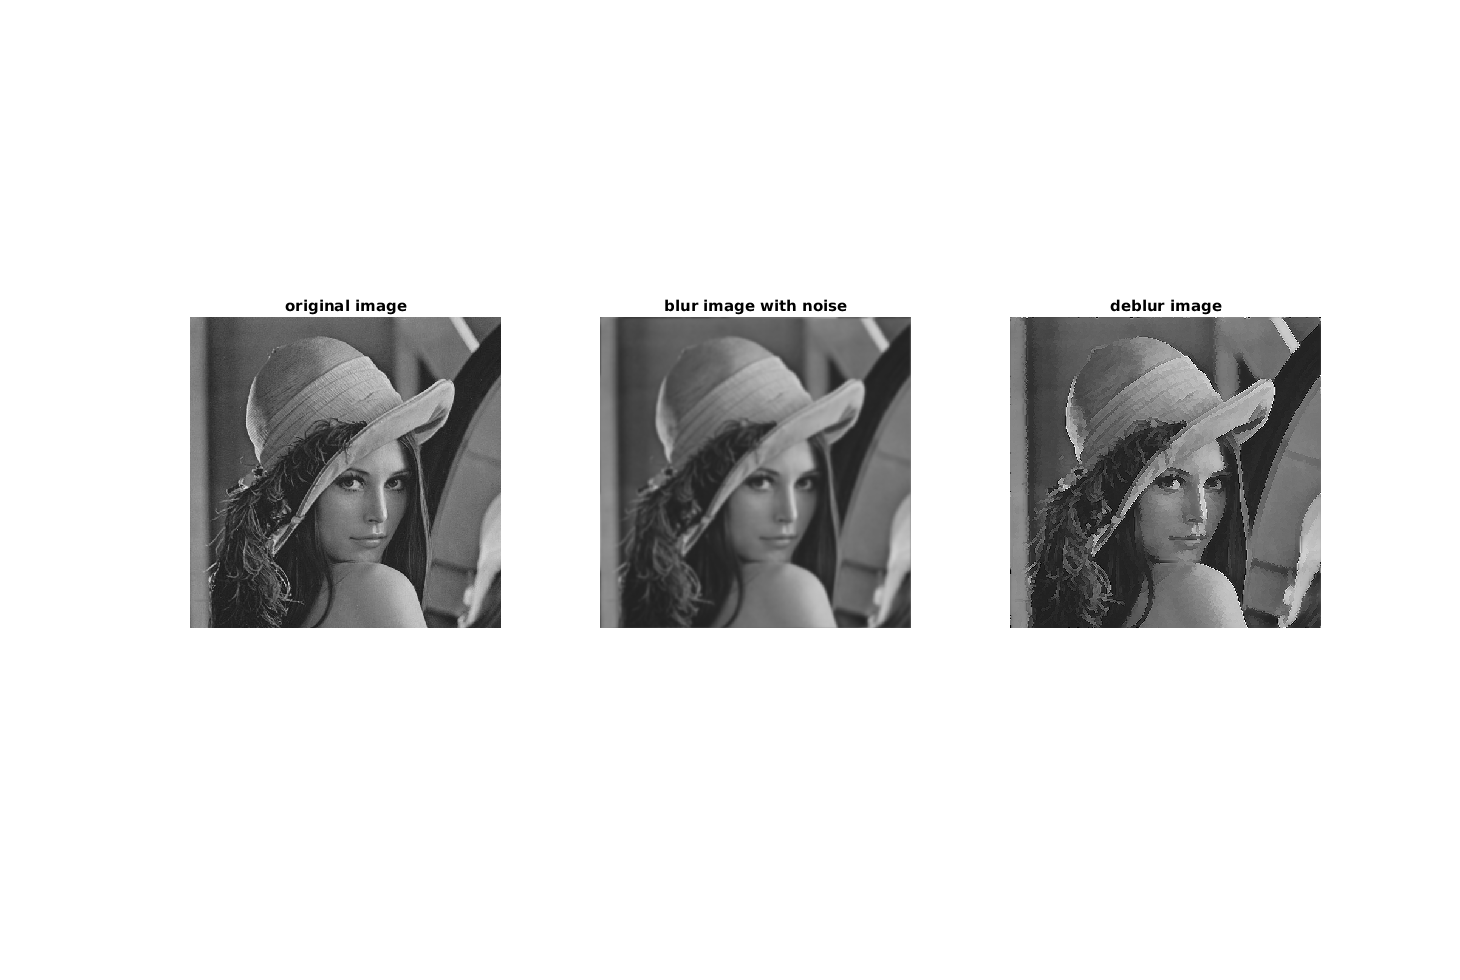
\includegraphics[width=0.8\textwidth]{hw2_fig5.png}
					\caption{shock\_filter\_deblur数值实验结果}
					\label{}
				\end{figure}
				\begin{figure}[htbp!]
					\centering
					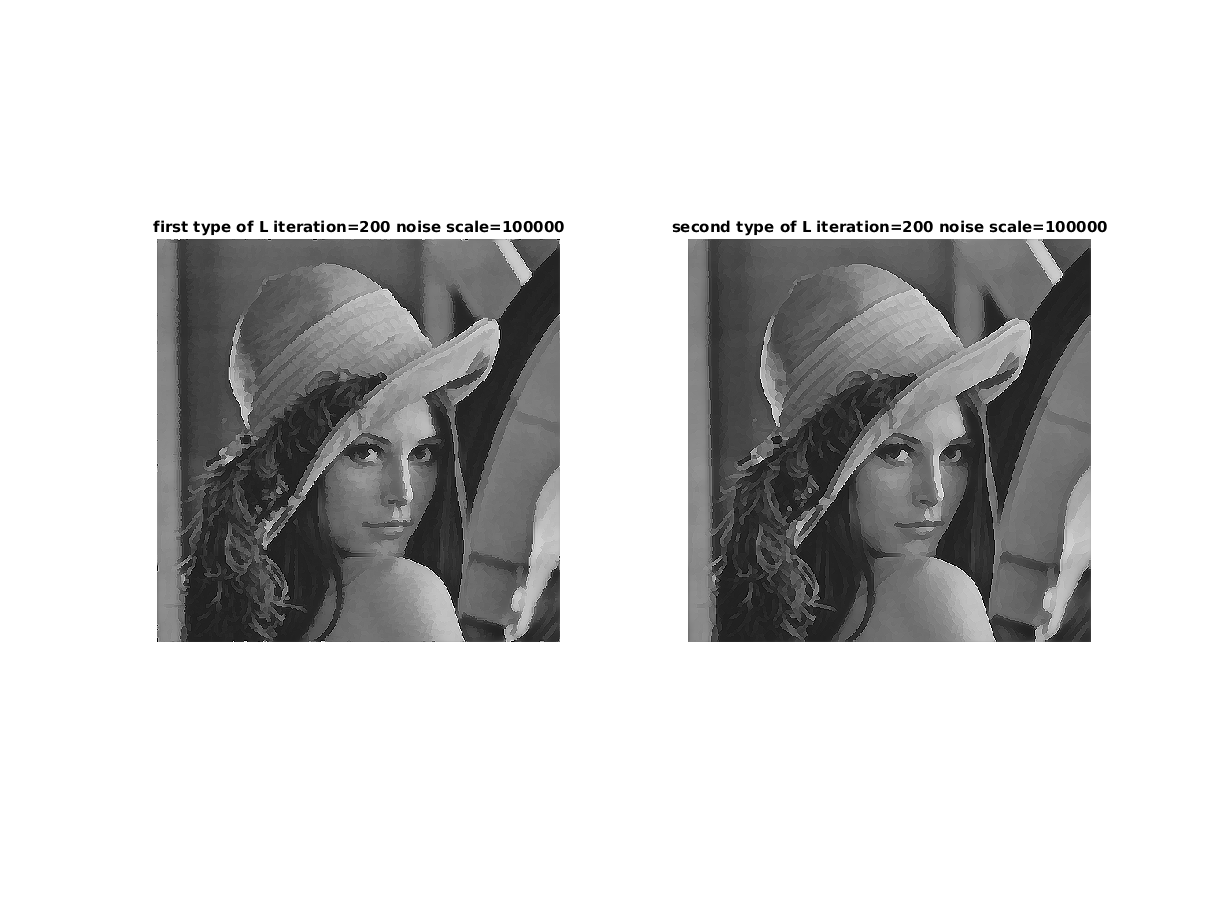
\includegraphics[width=0.8\textwidth]{hw2_fig6.png}
					\caption{shock\_filter\_deblur数值实验结果}
					\label{}
				\end{figure}
				\begin{figure}[htbp!]
					\centering
					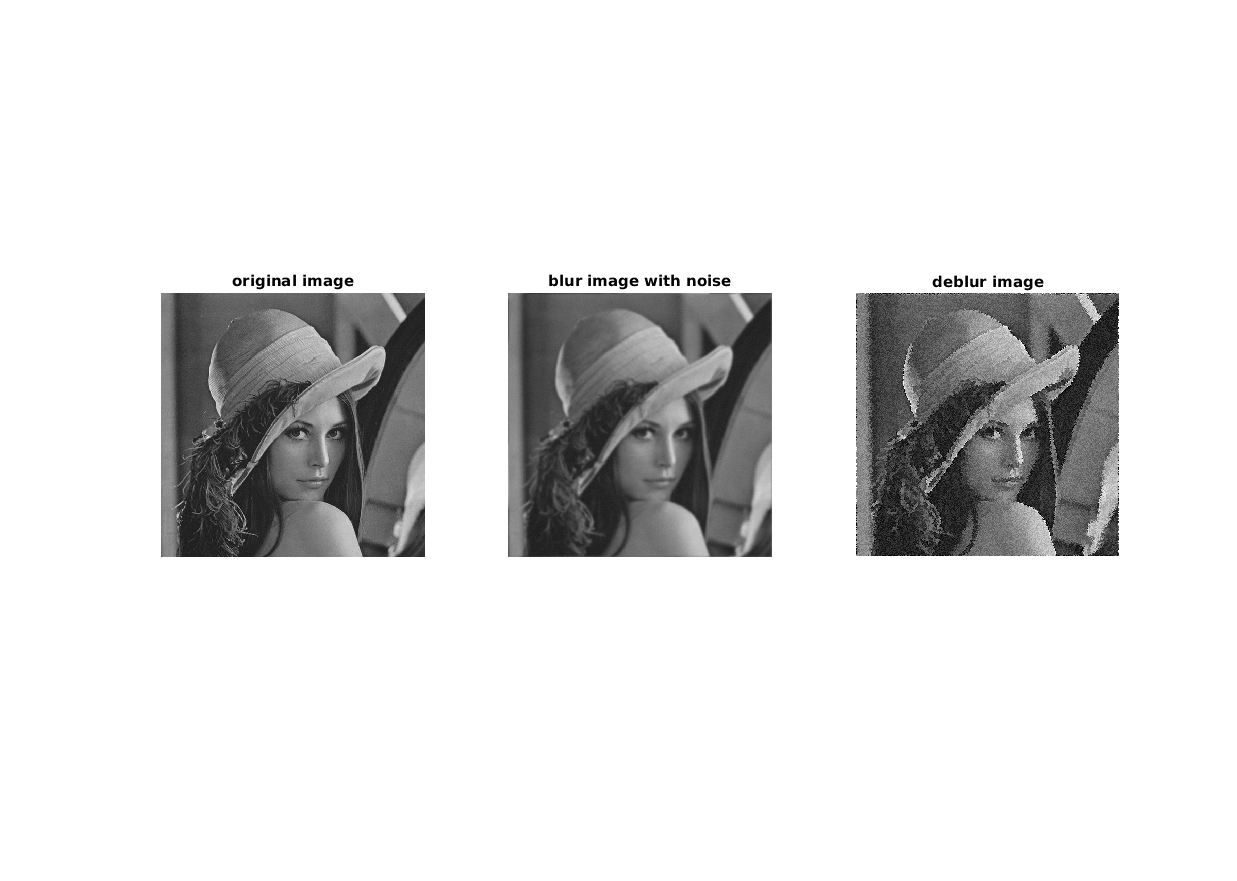
\includegraphics[width=0.8\textwidth]{hw2_fig7.png}
					\caption{shock\_filter\_deblur数值实验结果}
					\label{}
				\end{figure}
				\begin{figure}[htbp!]
					\centering
					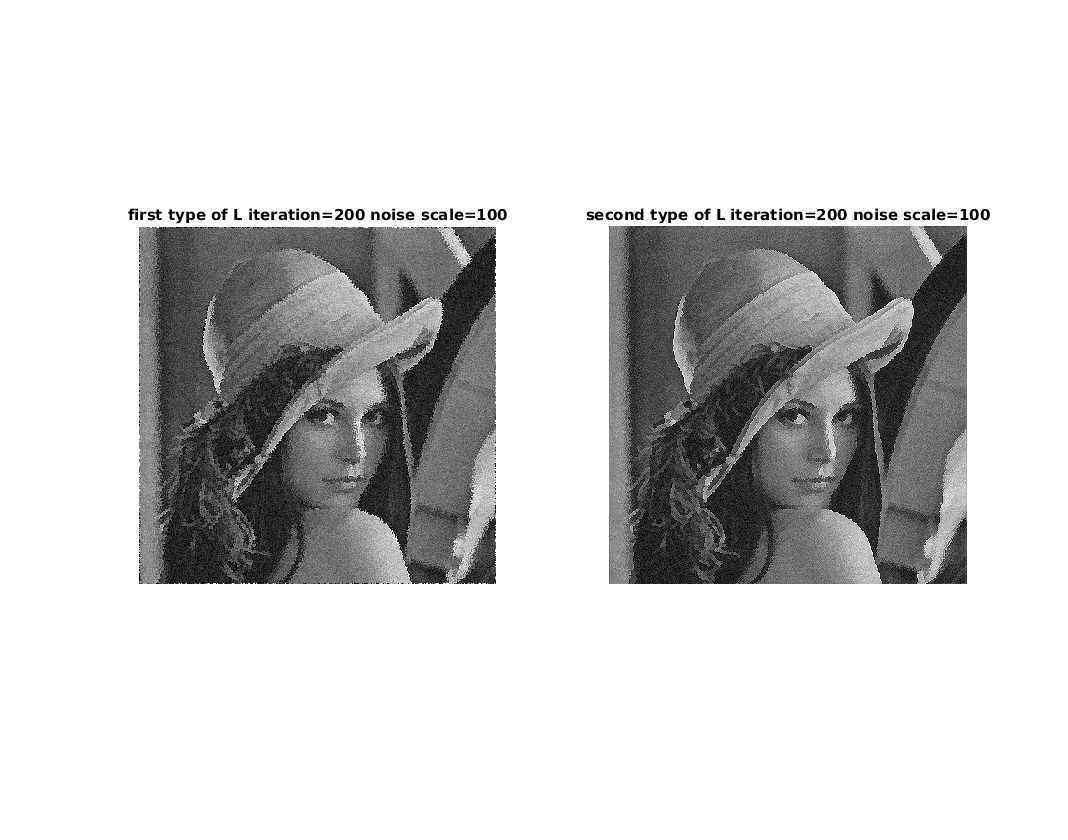
\includegraphics[width=0.8\textwidth]{hw2_fig8.png}
					\caption{shock\_filter\_deblur数值实验结果}
					\label{}
				\end{figure}
				\begin{figure}[htbp!]
					\centering
					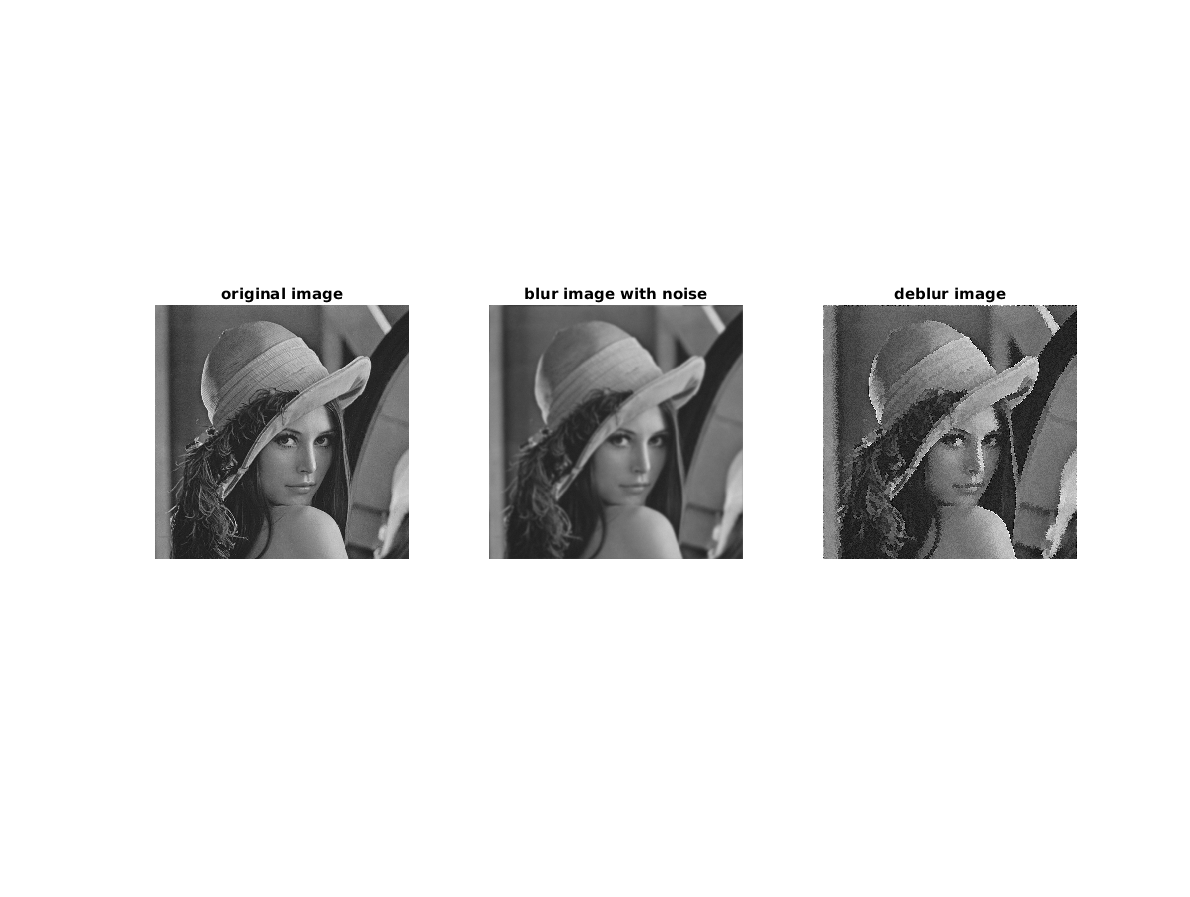
\includegraphics[width=0.8\textwidth]{hw2_fig9.png}
					\caption{shock\_filter\_deblur数值实验结果}
					\label{}
				\end{figure}
				\begin{figure}[htbp!]
					\centering
					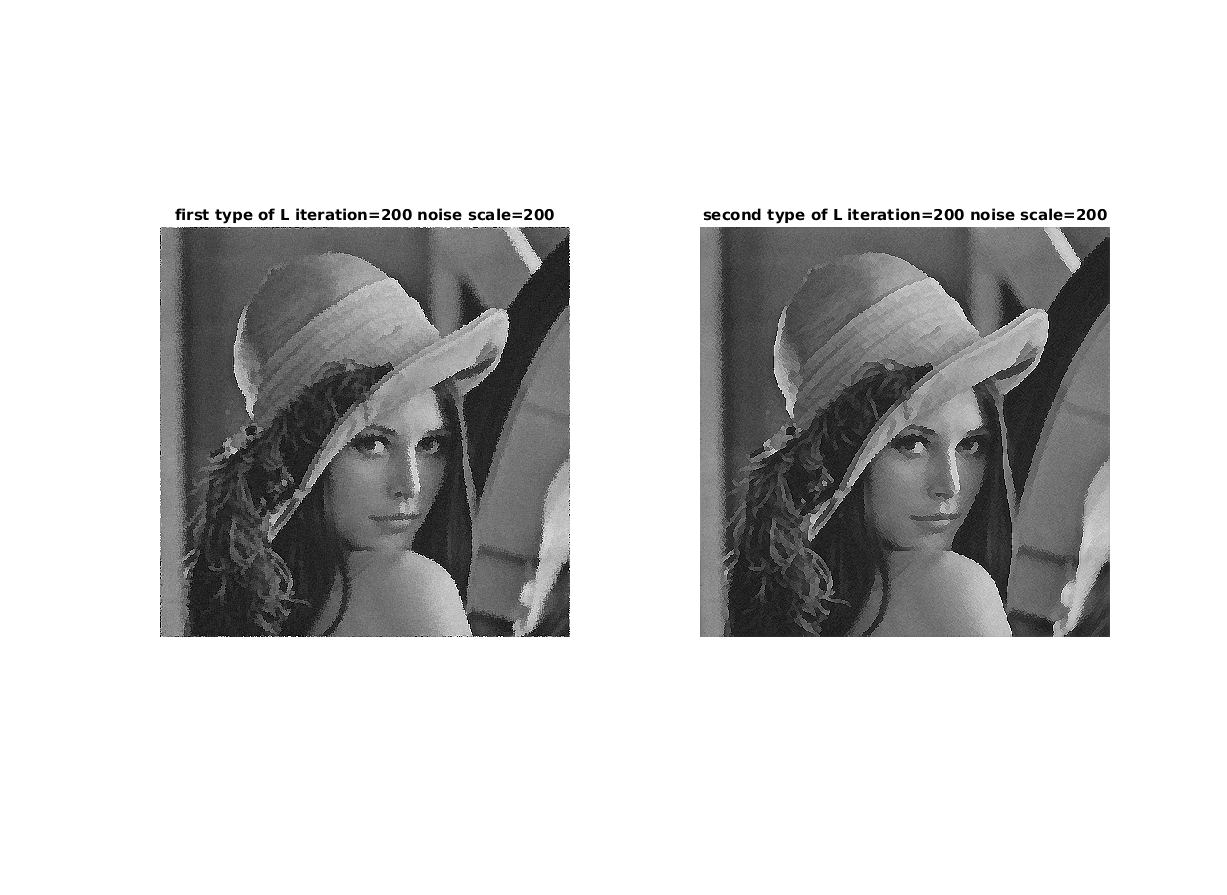
\includegraphics[width=0.8\textwidth]{hw2_fig10.png}
					\caption{shock\_filter\_deblur数值实验结果}
					\label{}
				\end{figure}
				\begin{figure}[htbp!]
					\centering
					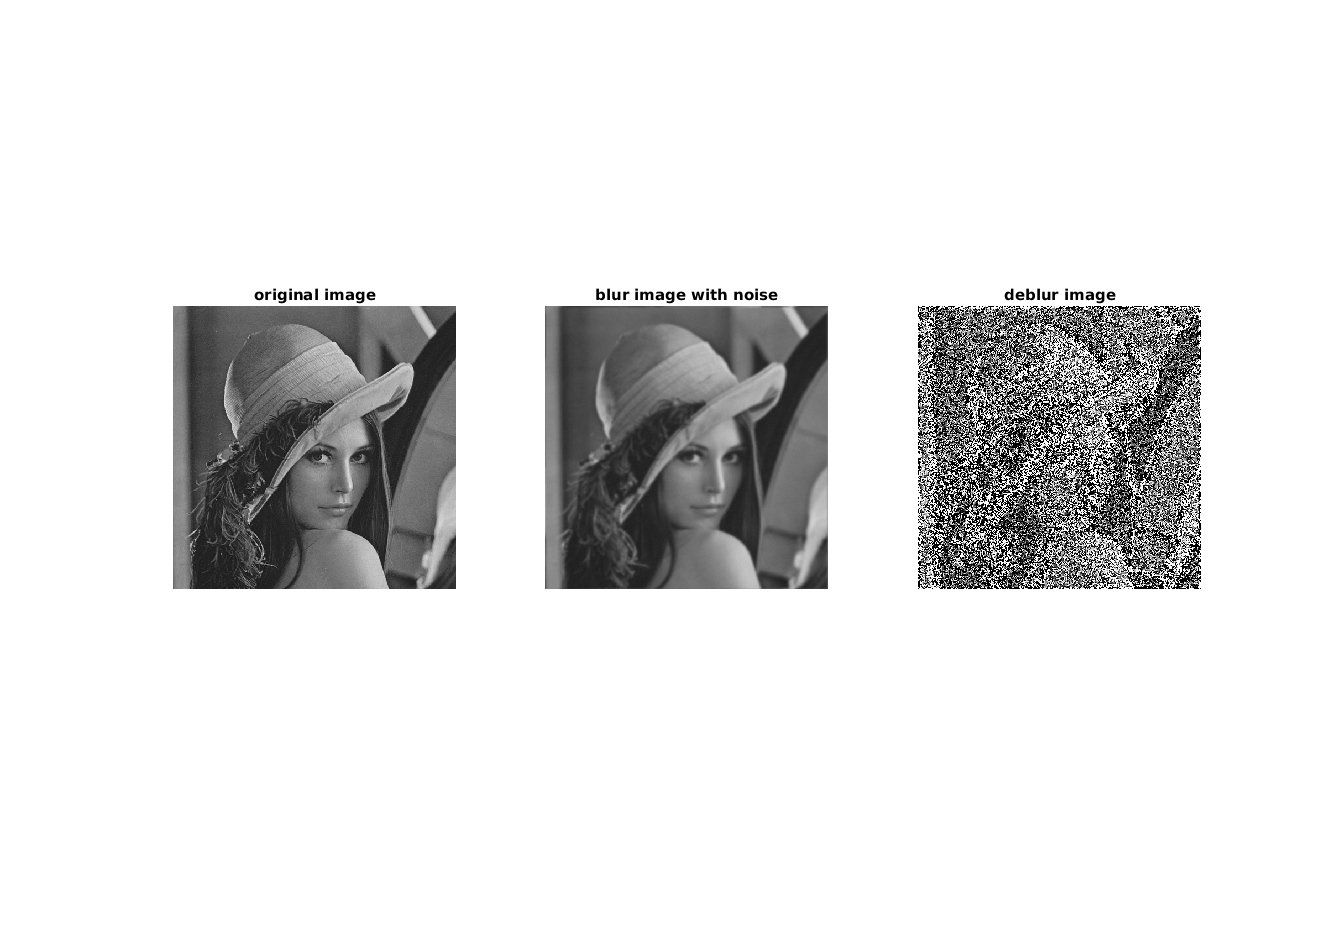
\includegraphics[width=0.8\textwidth]{hw2_fig11.png}
					\caption{shock\_filter\_deblur数值实验结果}
					\label{}
				\end{figure}
				\begin{figure}[htbp!]
					\centering
					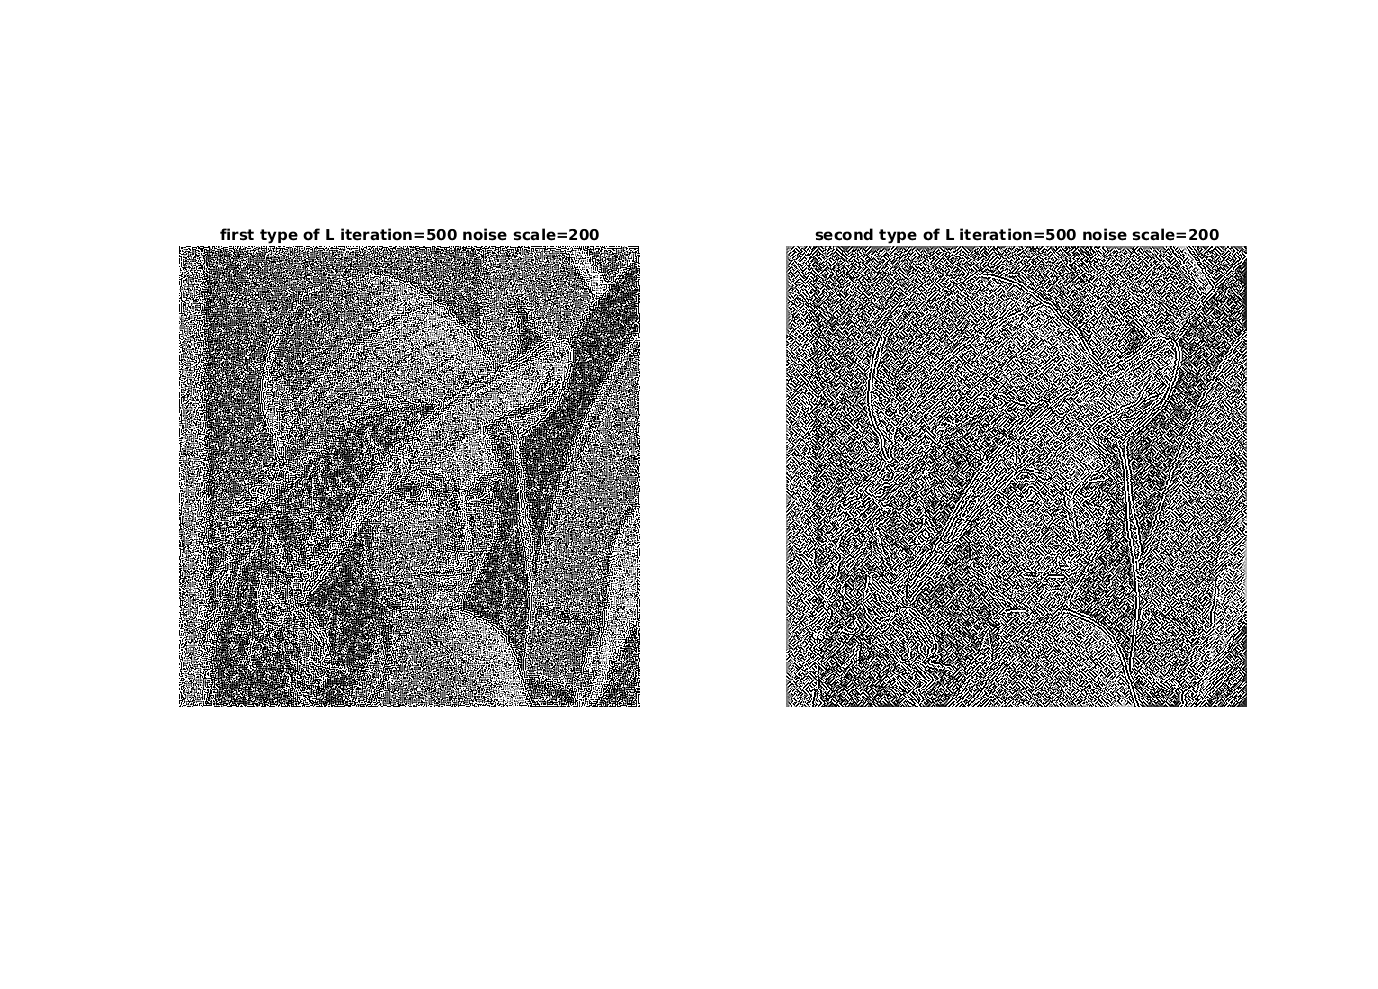
\includegraphics[width=0.8\textwidth]{hw2_fig12.png}
					\caption{shock\_filter\_deblur数值实验结果}
					\label{}
				\end{figure}
				\begin{figure}[htbp!]
					\centering
					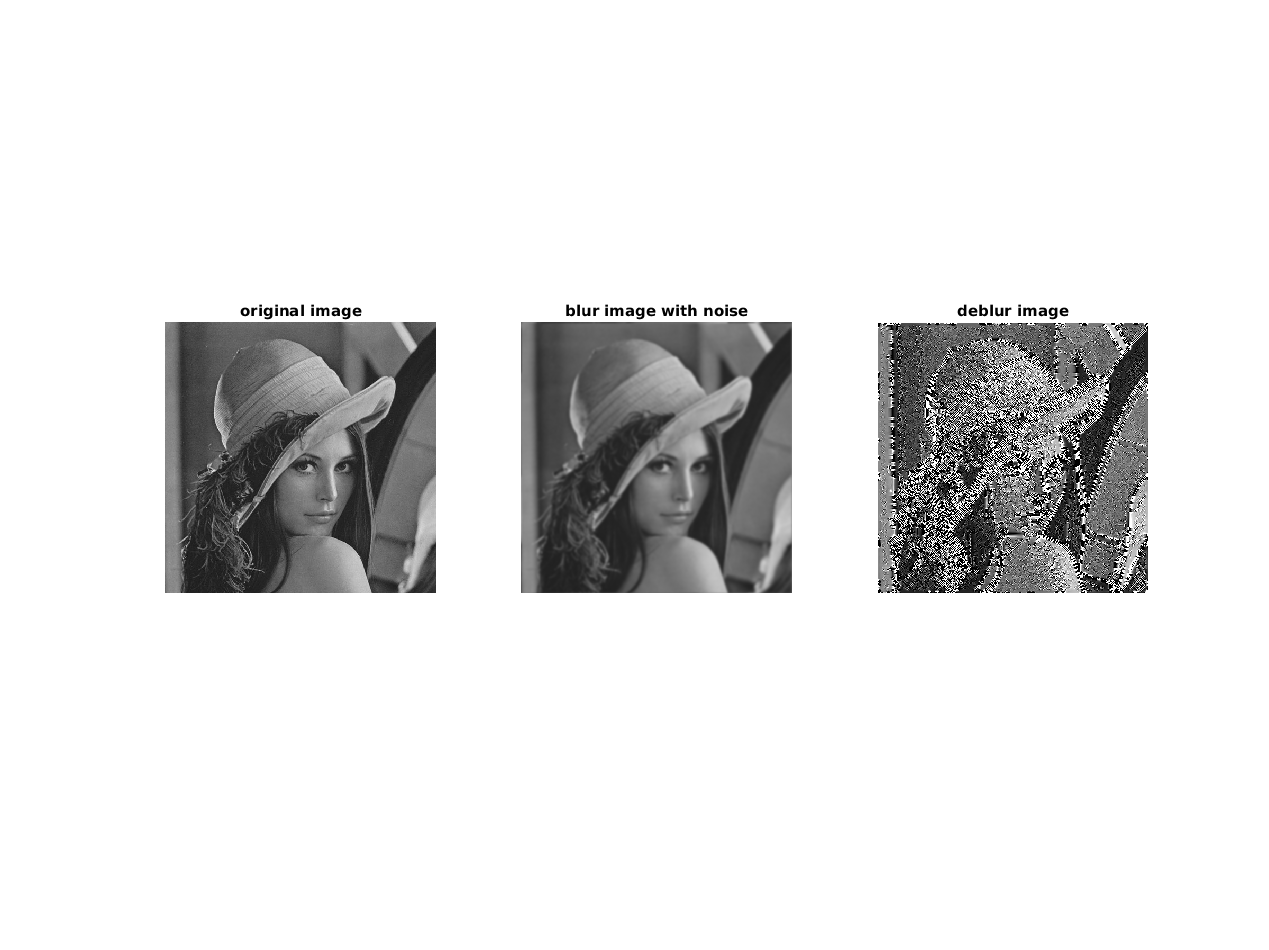
\includegraphics[width=0.8\textwidth]{hw2_fig13.png}
					\caption{shock\_filter\_deblur数值实验结果}
					\label{}
				\end{figure}
				\begin{figure}[htbp!]
					\centering
					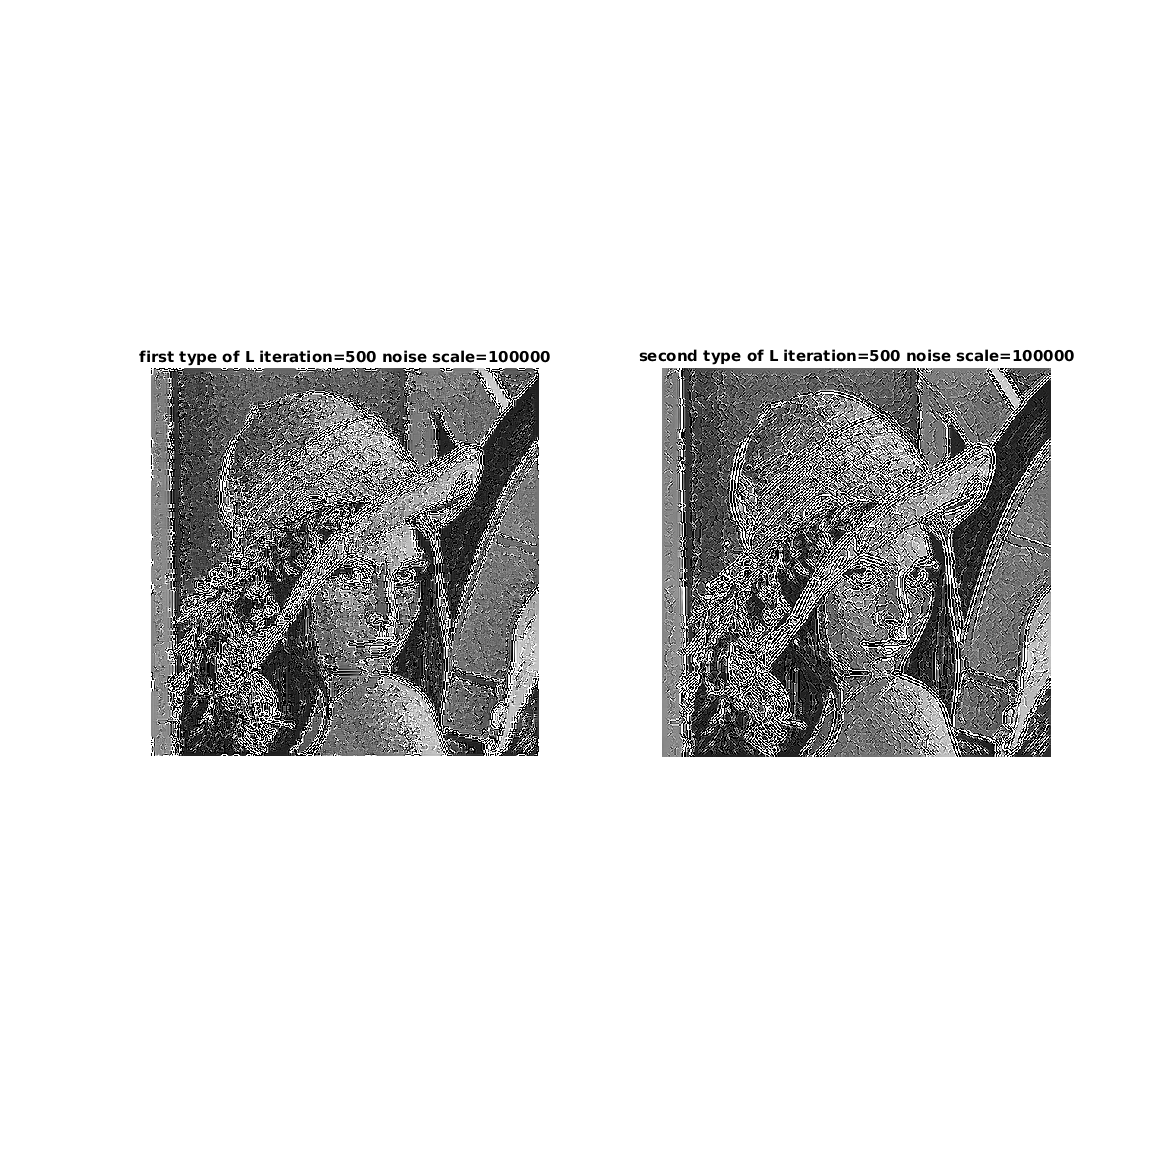
\includegraphics[width=0.8\textwidth]{hw2_fig14.png}
					\caption{shock\_filter\_deblur数值实验结果}
					\label{}
				\end{figure}
				\clearpage
		\section{结论}
			从上述数值实验过程,可以得到以下结论:
			\begin{enumerate}
				\item heat equation和perona malik算法随着演化时间变长,图像会越来越平滑,细节丢失越来越严重,这与老师上课讲到的结论是相同的;
				\item heat equation和perona malik算法相比,效果较差,perona malik算法可以在去噪的同时更好的保留图像的边缘信息,使得去噪之后的图像在观感上更好;
				\item shock filter算法在没有噪声的情况下,可以很好的增强图像的边缘信息,即实现模糊图像的锐化,但是,对于噪声图像,shock filter在增强边缘细节的同时也会增强噪声的信息,图像会受到更大噪声的影响;
				\item shock filter算法中的两种L算子,第二种明显在细节的增强上要优于第一种,且在噪声图像上有更好的表现;
				\item shock filter算法在长时间演化下会产生非常奇特的现象,可以从数值实验的结果看出,图像显得很乱,仔细看会发现:对于没有噪声的图像,shock filter算法过度增强了图像的边缘,导致图像边缘太过于突出;对于含噪图像,shock filter算法在过度增强边缘的同时,还过度增强了噪声,使得图像中出现了雪花点一般的噪声。产生上述结果说明了在长期演化的情况下,shock filter算法没有稳定收敛的解;
			\end{enumerate}

\end{document}
